\documentclass[10pt, titlepage, oneside, a4paper]{article}
\usepackage{array}
\usepackage{caption}
\usepackage{fancyhdr}
\usepackage{graphicx}
\usepackage{hyperref}
\usepackage{indentfirst}
\usepackage{lastpage}
\usepackage{lmodern}
\usepackage[utf8]{inputenc}
\usepackage{polski}

\graphicspath{ {./images/} }
\urlstyle{same}

\title{Specyfikacja Projektu ,,Expert4Home''}
\author{K. Dąbrowski, J. Grygiel, S. Kalisz\\
K. Malinowski, P. Piętka, B.Zdrojewski}
\date{Wersja 1.0\\\today}

\pagestyle{fancy}
\fancyhf{}
\lhead{Specyfikacja Projektu ,,Expert4Home''}
\rhead{Wersja 1.0}
\rfoot{\thepage \hspace{1pt} / \pageref{LastPage}}

\begin{document}

	\maketitle
	\thispagestyle{empty}  
	\newpage
  
	\section{Wstęp} 
  
	\subsection{Cel dokumentu}
	Celem dokumentu jest klarowne przekazanie propozycji realizacji celu projektu. W dokumencie zaprezentowano podstawy \textbf{architektury systemu}, które będą rozwijane i uszczegóławiane wraz z postępem projektu, schematy elementów \textbf{interfejsu użytkownika}, niezbędnych do realizacji kluczowych funkcji systemu, sugerowane \textbf{technologie}, które, na stan wiedzy autorów, wydają się być najlepiej dopasowane do skali i celów projektu, oraz \textbf{metody organizacji pracy}, wraz z \textbf{harmonogramem prac}, które mają zapewnić, że projekt zostanie ukończony w wyznaczonych ramach czasowych.
  
	\subsection{Cel projektu}
	Celem projektu jest zaprojektowanie i zaimplementowanie aplikacji webowej, której przeznaczeniem będzie łączenie specjalistów z danej branży z potencjalnymi klientami. 
	
	Z punktu widzenia specjalisty, aplikacja będzie pozwalać na publikację profilu dowolnej działalności, opartej o realizację usług lub zleceń, oraz zapewniać platformę do kontaktu z klientami.
	
	Natomiast z punktu widzenia klienta, aplikacja będzie pozwalać na wyszukanie specjalisty, skontaktowanie się z nim, ustalenie szczegółów usługi lub zlecenia, a ostatecznie na wyrażenie opinii na temat jakości wykonanej przez niego usługi lub zlecenia.
  
	\subsection{Użytkownicy końcowi}
	Użytkownikami końcowymi mogą być zarówno specjaliści, którzy chcą poszerzyć zasięg swojej działalności lub ułatwić komunikację na linii przedsiębiorca-klient, jak i dowolne osoby poszukujące sprawdzonych i dostosowanych do ich potrzeb usługodawców i zleceniobiorców.
	\newpage  
  
	\section{Architektura systemu}
  
  \subsection{Aktorzy}
	Osoby korzystające z aplikacji będą mogły grać rolę różnych aktorów podczas interakcji z systemem w zależności od celu, który chcą osiągnąć.
	Oznacza to, że ta sama osoba może raz wystąpić w roli eksperta oferującego swoje usługi, a innym razem skorzystać z systemu jako klient szukający wykonawcy zlecenia.

	\subsubsection*{Lista przewidzianych aktorów}
	\begin{itemize}
		\item Ekspert -- Osoba posiadająca wiedzę i umiejętności w danej dziedzinie pozwalające na świadczenie usług innym,
		\item Klient -- Osoba szukająca wykonawcy usług
		\item Stały klient -- Klient, który nawiązał wielokrotną w spółpracę z \textbf{konkretnym ekspertem}. Ma on dostęp do dodatkowych benefitów udzielonych przez eksperta
		\item Administrator -- Osoba mająca dodatkowe uprawnienia dzięki którym może wypływać na działanie systemu dla zwykłych użytkowników
	\end{itemize}
	
  \subsection{Przypadki użycia}
  Diagram przypadków użycia przedstawia rysunek \ref{fig:ucDiagram}.

  \begin{figure}[h]
	  \centering
	  \includegraphics[width=0.8\textwidth{}]{use_case_diagram.png}
	  \caption{Diagram przypadków użycia}
	  \label{fig:ucDiagram}
  \end{figure}
  
  \subsection{Diagramy sekwencji}
	todo kd tak jak na uml'u, na jednym diagramie (użyć \url{https://draw.io}, projekt zapisać w schemes, obraz wyeksportować do images, obraz wstawić z podpisem) przedstawić proces wyszukania specjalisty, dodania zgłoszenia, zaakceptowania zgłoszenia przez specjalistę i wystawienia komentarza, na podstawie zdjęć ze slackowego hash tag frontend (zdaję sobię sprawę, że wyciągnięcie procesu ze zdjęć widoków może być nieoczywiste, więc w razie czego pisz do bz/jg/sk)
	\newpage
  
	\section{Interfejs użytkownika}
  
	\subsection{Ekran główny}
	\begin{figure}[!htbp]
  \begin{center}
  {%
		\setlength{\fboxsep}{0.5pt}%
		\setlength{\fboxrule}{0.5pt}%
		\fbox{
			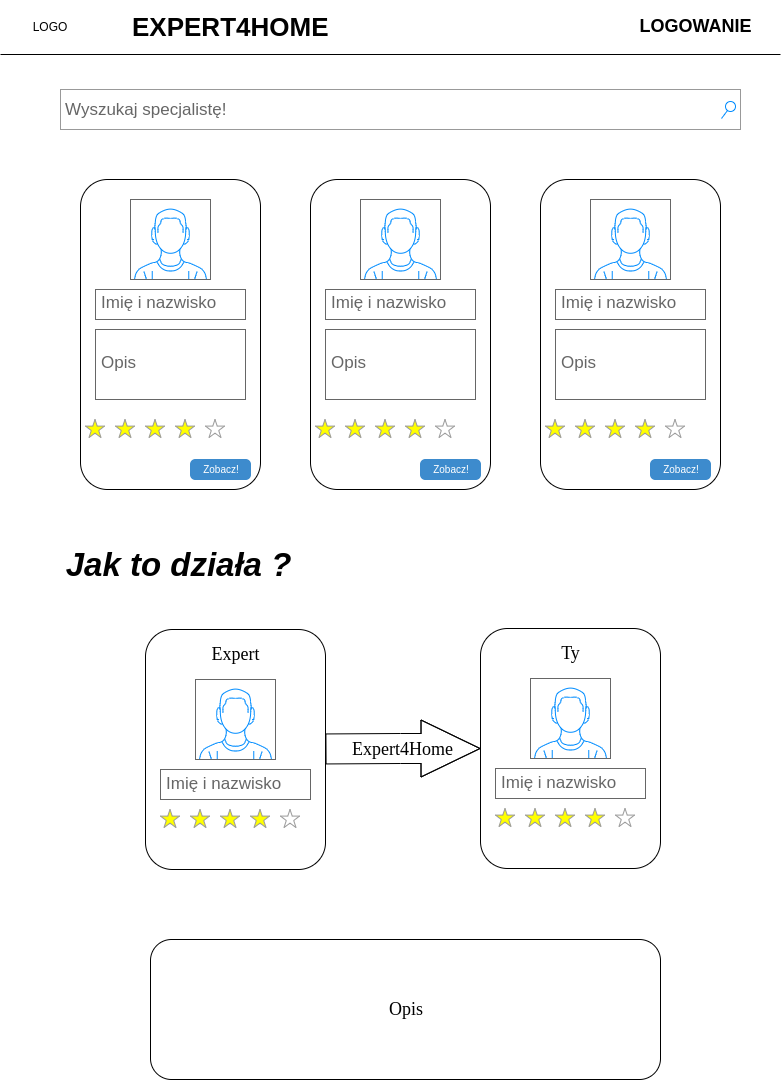
\includegraphics[width=\textwidth]{home_view.png}
		}%
	}%
  \captionof{figure}{Schemat ekranu głównego}
  \end{center}
  \end{figure}
	\newpage

	\subsection{Ekran wyszukiwania specjalisty}
	\begin{figure}[!htbp]
  \begin{center}
  {%
		\setlength{\fboxsep}{0.5pt}%
		\setlength{\fboxrule}{0.5pt}%
		\fbox{
			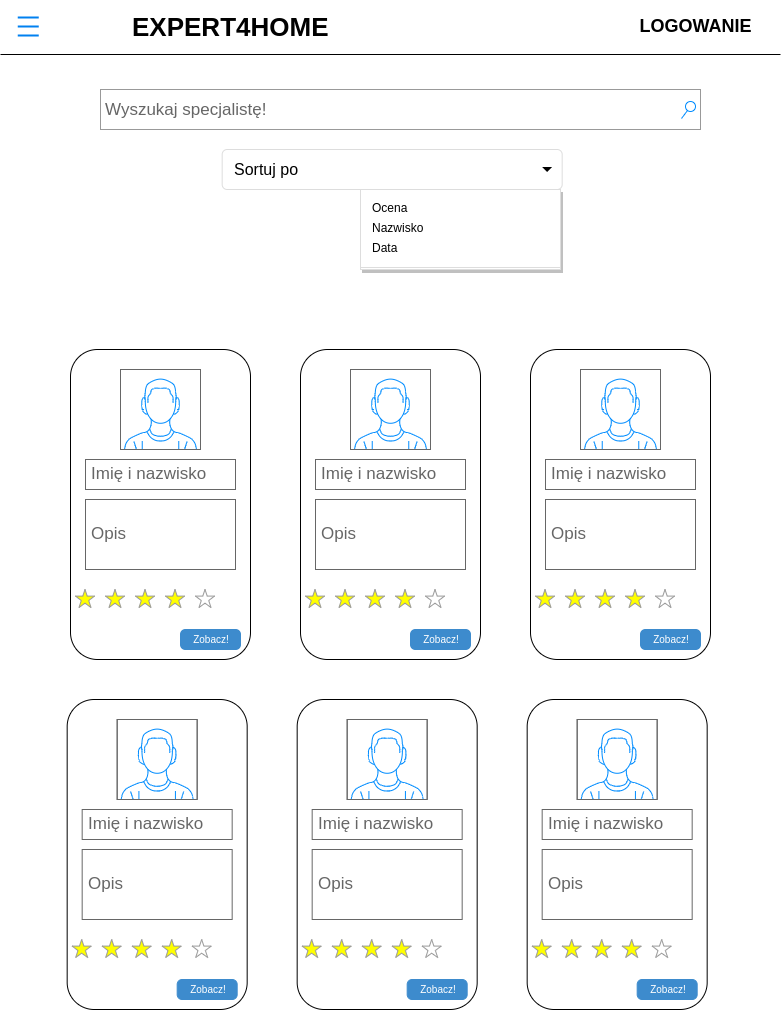
\includegraphics[width=\textwidth]{search_expert_view.png}
		}%
	}%
  \captionof{figure}{Schemat ekranu wyszukiwania specjalisty}
  \end{center}
  \end{figure}
	\newpage

	\subsection{Ekran profilu specjalisty}	
	\begin{figure}[!htbp]
  \begin{center}
  {%
		\setlength{\fboxsep}{0.5pt}%
		\setlength{\fboxrule}{0.5pt}%
		\fbox{
			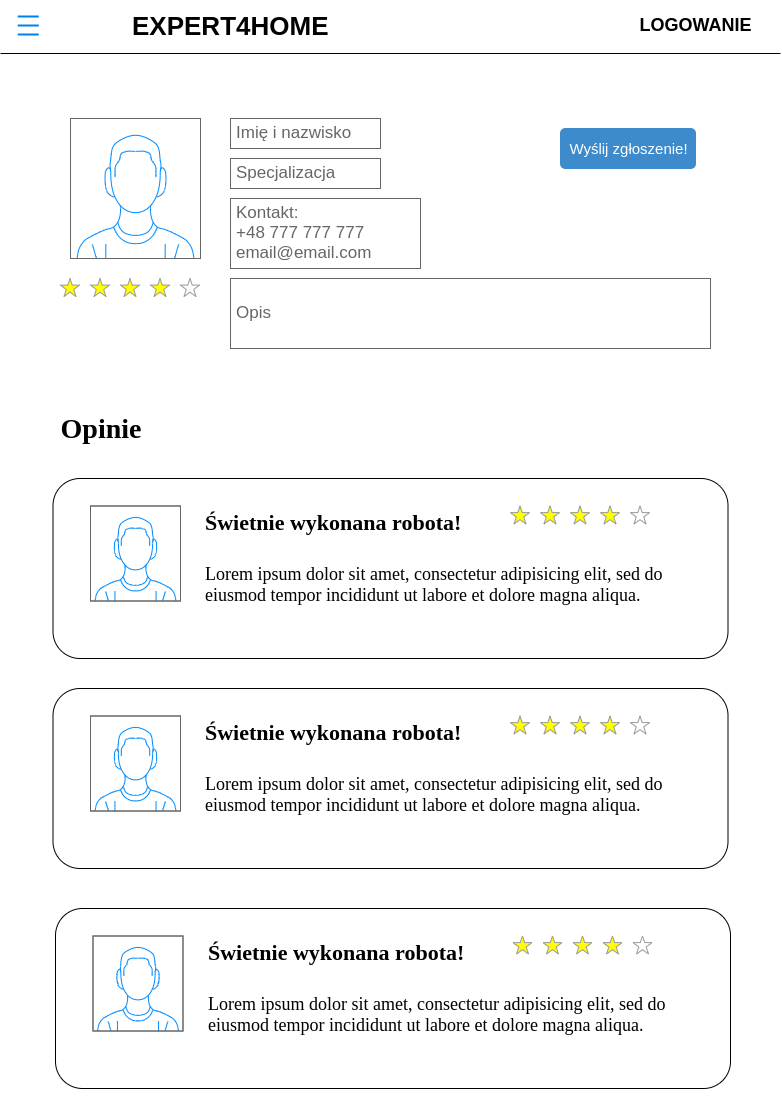
\includegraphics[width=\textwidth]{expert_profile_view.png}
		}%
	}%
  \captionof{figure}{Schemat ekranu profilu specjalisty}
  \end{center}
  \end{figure}
	\newpage
	
	\subsection{Dialog zgłoszenia}	
	todo sk przerysować w \url{https://draw.io} ze slackowego hash tag frontend, zapisać projekt do schemes, wyeksportować obraz do images, wstawić obraz tutaj z podpisem	
	\newpage	
	
	\subsection{Ekran zgłoszeń klienta}
	todo sk przerysować w \url{https://draw.io} ze slackowego hash tag frontend, zapisać projekt do schemes, wyeksportować obraz do images, wstawić obraz tutaj z podpisem
	\newpage	
	
	\subsection{Ekran zgłoszeń specjalisty}
	todo sk przerysować w \url{https://draw.io} ze slackowego hash tag frontend, zapisać projekt do schemes, wyeksportować obraz do images, wstawić obraz tutaj z podpisem  
	\newpage  
  
	\section{Szczegóły implementacji}  
  
	\subsection{Środowisko deweloperskie}  
	Jednym z ważniejszych wyzwań jest zapewnienie spójności środowisk pomiędzy uczestnikami zespołu. Wszelkie
	nawet najmniejsze odchylenia mogą prowadzić do błędów, co gorsza większość problemów może być nie możliwa
	do odtworzenia na innych maszynach. Ponieważ wybraliśmy javę 8 jako język programowania niezbędna jest
	automatyzacja budowania oraz zarządzania zależnościami itp. Postanowiliśmy użyć programu gradle Gradle,
	posiada on prostą i przejrzystą składnie ułatwiającą pracę. Mimo ułatwienia jakim jest Gradle, nie jest
	wystarczającym środkiem zapewnienia spójności. W celu osiągnięcia jej postanowiliśmy skorzystać z
	kontenerów Dockerowych. Ze względu na rozmiar kontenerów Windowsowych, jedyną możliwą opcją są kontenery
	Linuxowe. Oznacza to iż platformą docelową dla każdego fragmentu aplikacji jest Alpine Linux. Konteneryzacja
	aplikacji ułatwia również późniejsze uruchomienie jej w środowisku chmurowym. Każdy z 3 najpopularniejszych
	dostawców oferuje hosting dla kontenerów.
  
	\subsection{Zastosowane technologie}

	\subsubsection{Front-end}
	todo jg+sk react
	
	\subsubsection{Back-end}	
	Do serwerowej części projektu postanowiliśmy wykorzystać kilka technologii. Zostaną one opisane poniżej.
	
	\paragraph{SpringBoot} \mbox{} \par
	Do napisania kodu części serwerowej aplikacji wybraliśmy framework \texttt{SpringBoot} języka \texttt{Java}.
	Jest to rozwiązanie sprawdzone przez wiele firm i rozwijane oraz wspierane już przez wiele lat. Dzięki temu możemy korzystać z dopracowanych bibliotek oraz zdobyć cenne doświadczenie.

	\texttt{SpringBoot} jest bazowany na frameworku \texttt{Spring} jednak w przeciwieństwie do niego znacznie ogranicza niepotrzebną konfigurację na rzecz konwencji.
	Dzięki takiemu podejściu programista może skupić się na realizowaniu funkcjonalności zamiast na przygotowywaniu środowiska.

	\paragraph{Tomcat} \mbox{} \par
	Do uruchomienia aplikacji oraz obsługi połączeń sieciowych zastosowany został serwer \texttt{Tomcat}.
	Jest to rozwiązanie o otwartym kodzie źródłowym wspierane przez organizację Apache.
	Stanowi domyślne rozwiązanie dla aplikacji sieciowych pisanych w języku Java.

	\paragraph{MySQL} \mbox{} \par
	Do przechowywania danych biznesowych aplikacji wybraliśmy bazę MySQL.
	Ponieważ dane maja wyraźną strukturę uznaliśmy, że rozwiązanie oparte na SQL będzie dobrze rozwiązywało problemy związane ze składowaniem danych.
	Baza \texttt{MySQL} posiada otwarty kod źródłowy, ma zaimplementowane wszystkie najważniejsze funkcjonalności silników bazodanowych takie jak transakcje, widoki czy wyzwalacze i jest to szeroko używane i sprawdzone rozwiązanie.

	\paragraph{Nginx} \mbox{} \par
	Przez wiele lat dominującym serwerem http na rynku był Apache. W 2019 został on zdetronizowany przez Nginxa. 
	Zdecydowaliśmy się użyć nowego króla. Głównych jego cechą jest możliwość obsługiwania bardzo dużej liczby
	połączeń jednocześnie, dzięki asynchronicznemu podejściu do obsługi zapytań. Apache obsługuje połączenia
	synchronicznie, tj. tworzy nowy proces dla każdego połączenia. Ponad to składnia konfiguracji Nginx jest
	znacznie bardziej przejrzysta niż konfiguracja Apache. Dodatkową zaletą Nginxa jest jego popularność. Oznacza
	to iż w sytuacji natrafienia na trudności istnieje duża szansa iż ktoś już kiedyś natrafił na podobny problem.
	
	\subsubsection{Kontrola wersji}
	W celu zapewnienia możliwości monitorowania i wycofywania zmian w kodzie źródłowym aplikacji oraz równoległej, bezkonfliktowej pracy wszystkich członków zespołu, postanowiono skorzystać z systemu kontroli wersji. Wybrano znany i szeroko stosowany system \textbf{git}. Dodatkowo, w celu zapewnienia łatwego dostępu do repozytorium aplikacji, postanowiono skorzystać z serwisu \textbf{Github}.
	
	Repozytorium składać się będzie z co najmniej dwóch gałęzi: \textit{master} i \textit{development}. Na gałęzi \textit{development} będą prowadzone prace deweloperskie. Wszelkie dodatkowe gałęzie, które zostaną stworzone na potrzeby konkretnych funkcjonalności, będą łączone właśnie z tą gałęzią.
	
	Gdy wszystkie zmiany na gałęzi \textit{development} zostaną przetestowane i stabilność danej wersji aplikacji zostanie potwierdzona, zostaną one połączone z gałęzią \textit{master}.
	  
	\subsubsection{Wdrożenie oprogramowania}
	Istnienie kontenerów Dockerowy otwiera przed naszym zespołem wiele nowych możliwości. Dzięki sposobowi dystrybucji
	jakim jest Docker Hub w bardzo prosty sposób można uzyskać dostęp do wielu jż stworzonych obrazów dysków. Możliwym
	jest również rozstawienie własnego rejestru obrazów. W efekcie pobieranie wszelkiego rodzaju zależności sprowadza
	się do jednej komendy, gdzie każda zależności "myśli" że jest oddzielnym systemem operacyjnym. Przykładowo,
	jeżeli potrzebujemy bazy postgreSQL wystarczy wywołać komendę \texttt{docker pull postgres}, odpowiedni obraz
	zostanie pobrany.
	
	Docelowo środowiskiem produkcyjnym aplikacji będzie chmura Microsoft Azure. Dokładnie oferowany przez MSA hosting
	kontenerów. Zdecydowaliśmy się na Azure ze względu na możliwość połączenia ponieważ korzystamy z pakietu Azure DevOps. 
	Azure Devops pozwala na zarządzanie zadaniami, hostowanie prywatnych rejestrów Dockerowych oraz co najważniejsze,
	pozwala na definiowanie procesów CI/CD. W odpowiednim etapie dojrzałości projektu planujemy skorzystać z właśnie
	tej funkcjonalności w celu usprawnienia całego procesu wytwarzania oprogramowania.

	  
	\subsection{Plan testów}	
	Ponieważ w projekcie ma być używana metodyka SCRUM, korzystanie z techniki TDD nie jest obowiązkowe. Mimo to 
	testy jednostkowe nadal okazują się przydatne. Pozwalają na pewnego rodzaju dokumentowanie kodu za pomocą testów,
	pozwalają zrozumieć celowość przykładowej metody, sposób wywoływania i jak działa bez wnikania w szczegóły kodu.
	Moze to się okazać przydatne/kluczowe, gdy piszemy kod do jeszcze nieistniejącej klasy/metody/funkcjonalności,
	a więc ułatwia w znaczący sposób zrównoleglenie pracy nad problemem.
	Testy jednostkowe zazwyczaj odnoszą się do klasy, lub metody, pokrywają możliwe scenariusze i sprawdzają czy metoda/klasa
	dobrze je obsłużyła. W razie gdy metoda polega na innej klasie, niż do tej, do której należy, stosuje się atrapę obiektu/ów (mock),
	która symuluje przy wywołaniu metody zwrócenie wartości, jaką mogłaby zwrócić prawdziwa funkcja. Testy jednostkowe narzucają
	w sposób niebezpośredni takiego pisania kodu, by ograniczyć te zależności, co jest zresztą dobrą praktyką.
	Testy integracyjne pozwalają już sprawdzić z zależnościami czy wszystko wypada dobrze. Moze mieć wiele potencjalnych
	punktów awarii, a nawet być zależny od konfiguracji. Dlatego są równie ważne. Dobre pokrycie kodu testami jednostkowymi
	jest w stanie przyspieszyć znalezienie błędu w testach integracyjnych. Jak widać, pisanie testów jest opłacalne, mimo tego, że
	nakłada pisania więcej kodu.
	\newpage 
 
	\section{Szczegóły organizacji pracy}  
 
	\subsection{Harmonogram prac}
	todo bz
 
	\subsection{Metodyka wytwarzania oprogramowania}
	todo sk scrum, kanban
	
	\subsection{Zastosowane narzędzia}
	todo kd azure devops, slack
 
\end{document}